\newpage
\section{Secchi Disk}\label{c:secchi-disk}

\subsection{Overview}\label{overview}

More information about Secchi DIsk can be found at:

  \URL{https://en.wikipedia.org/wiki/Secchi/_disk}

\begin{figure}[htb]
\centering
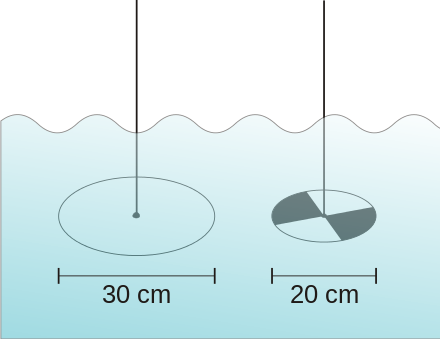
\includegraphics[height=0.25\textheight]{secchi/disk.png}
\caption{secchi}
\end{figure}

Figure: Different kinds of Secchi disks. A marine style on the left and
the freshwater version on the right {[}wikipedia{]}

\section{Setup for OSX}\label{setup-for-osx}

First lest setup the environment for OSX

\begin{verbatim}
import os, sys
from os.path import expanduser
os.path
home = expanduser("~")
sys.path.append('/usr/local/Cellar/opencv/3.3.1_1/lib/python3.6/site-packages/')
sys.path.append(home + '/.pyenv/versions/OPENCV/lib/python3.6/site-packages/')
import cv2
cv2.__version__
! pip install numpy > tmp.log
! pip install matplotlib >> tmp.log
%matplotlib inline
\end{verbatim}

\subsection{Step 1: Record the video}\label{step-1-record-the-video}

Record the video on the robot

\subsection{Step 2: Analyse the images from the
Video}\label{step-2-analyse-the-images-from-the-video}

For now we just selected 4 images from the video

\begin{verbatim}
import cv2
import matplotlib.pyplot as plt

img1 = cv2.imread('secchi/secchi1.png') 
img2 = cv2.imread('secchi/secchi2.png') 
img3 = cv2.imread('secchi/secchi3.png') 
img4 = cv2.imread('secchi/secchi4.png') 
\end{verbatim}

\begin{verbatim}
figures = []
fig = plt.figure(figsize=(18, 16))
for i in range(1,13):
    figures.append(fig.add_subplot(4,3,i))
count = 0
for img in [img1,img2,img3,img4]:
    figures[count].imshow(img)

    color = ('b','g','r')
    for i,col in enumerate(color):
        histr = cv2.calcHist([img],[i],None,[256],[0,256])
        figures[count+1].plot(histr,color = col)

    figures[count+2].hist(img.ravel(),256,[0,256])

    count += 3

print("Legend")
print("First column = image of Secchi disk")
print("Second column = histogram of colors in image")
print("Third column = histogram of all values")

plt.show() 
\end{verbatim}

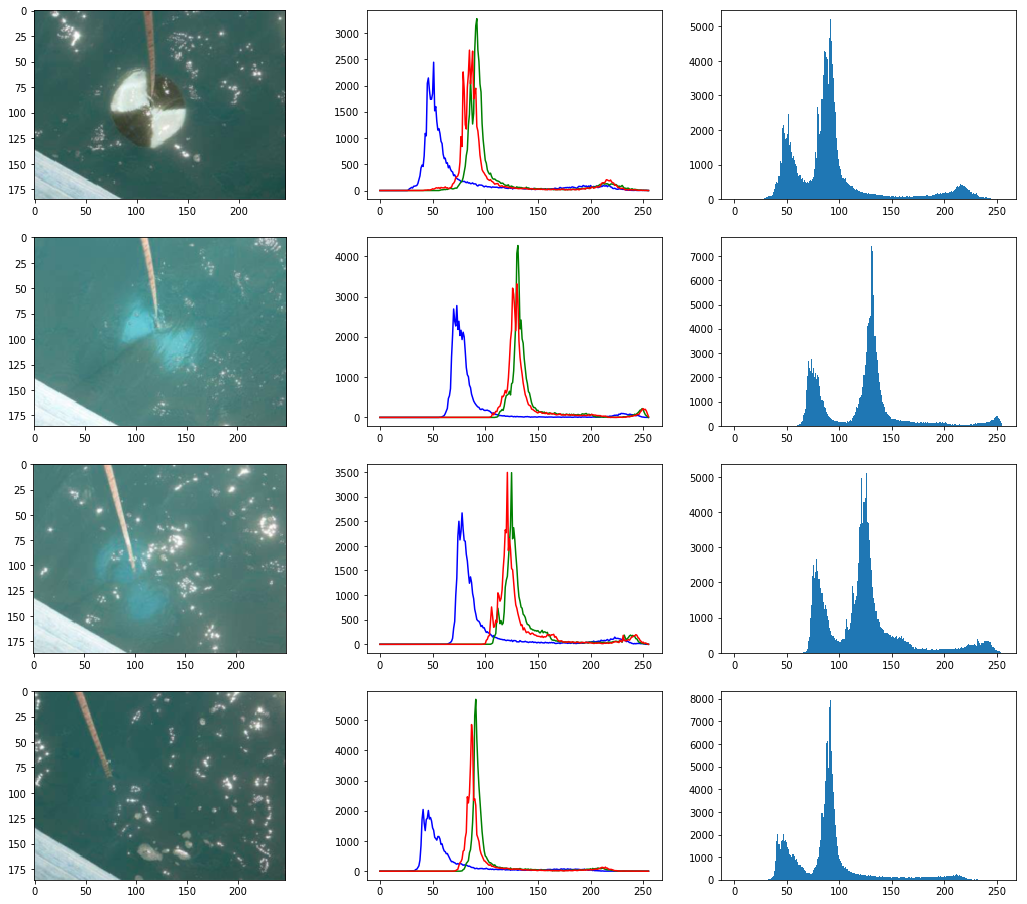
\includegraphics[width=1.0\textwidth]{secchi-a/output_9_1.png}

Rotation of the image for an angle of t

\subsubsection{Image Thresholding}\label{image-thresholding}

\begin{verbatim}
def threshold(img):
    ret,thresh = cv2.threshold(img,150,255,cv2.THRESH_BINARY)
    plt.subplot(1,2,1), plt.imshow(img, cmap='gray')
    plt.subplot(1,2,2), plt.imshow(thresh, cmap='gray')
\end{verbatim}

\begin{verbatim}
threshold(img1)
\end{verbatim}

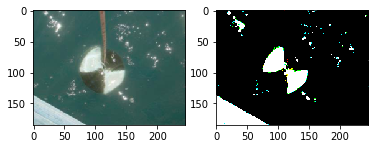
\includegraphics{secchi-a/output_13_0.png}


\begin{verbatim}
threshold(img2)
\end{verbatim}

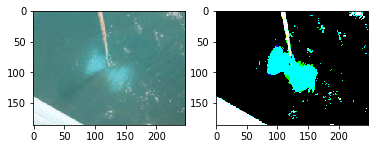
\includegraphics{secchi-a/output_14_0.png}

\begin{verbatim}
threshold(img3)
\end{verbatim}

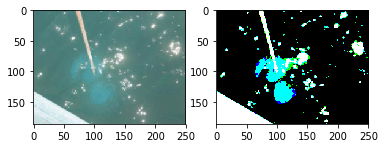
\includegraphics{secchi-a/output_15_0.png}

\begin{verbatim}
threshold(img4)
\end{verbatim}

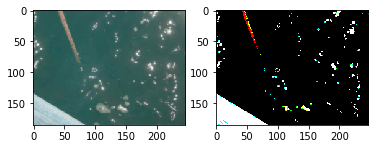
\includegraphics{secchi-a/output_16_0.png}

\subsubsection{Edge Detection}\label{edge-detection}

Edge detection using Canny edge detection algorithm

\begin{verbatim}
def find_edge(img):
    edges = cv2.Canny(img,50,200)
    plt.subplot(121),plt.imshow(img,cmap = 'gray')
    plt.subplot(122),plt.imshow(edges,cmap = 'gray')
\end{verbatim}

\begin{verbatim}
find_edge(img1)
\end{verbatim}

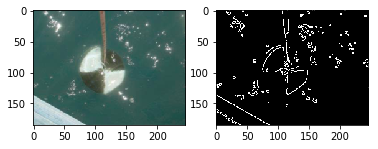
\includegraphics{secchi-a/output_19_0.png}

\begin{verbatim}
find_edge(img2)
\end{verbatim}

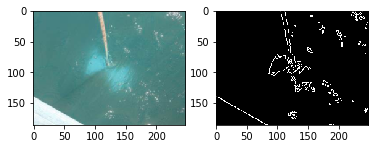
\includegraphics{secchi-a/output_20_0.png}

\begin{verbatim}
find_edge(img3)
\end{verbatim}

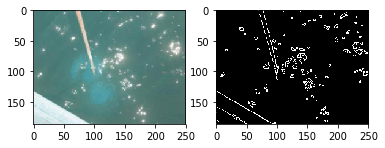
\includegraphics{secchi-a/output_21_0.png}

\begin{verbatim}
find_edge(img4)
\end{verbatim}

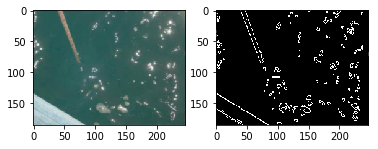
\includegraphics{secchi-a/output_22_0.png}

\section{Black and white}\label{black-and-white}

\begin{verbatim}
bw1 = cv2.cvtColor(img1, cv2.COLOR_BGR2GRAY)
plt.imshow(bw1, cmap='gray')
\end{verbatim}

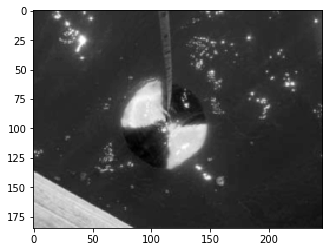
\includegraphics[width=0.5\textwidth]{secchi-a/output_26_1.png}
